%%% I wish this had bigger margins :(
\documentclass{llncs}

%%% basic packages %%%
\usepackage[T1]{fontenc} 
\usepackage{tgtermes}
\usepackage{amssymb}
\usepackage{amsmath}
\usepackage{graphicx}
\usepackage{esint}
\usepackage{enumitem}
\usepackage{algorithm}
\usepackage{hyperref}
\usepackage{marvosym}
\usepackage{mathtools}
\usepackage{xspace} 
\usepackage{color}

%%% some custom stuff %%%
\usepackage[noend]{algpseudocode}
\usepackage[section]{placeins}
\usepackage{hyperref}
\renewcommand\algorithmicthen{}
\renewcommand\algorithmicdo{}
\algrenewcommand\algorithmicindent{1.0em}
\newenvironment{megaalgorithm}[1][htb]
  {\renewcommand{\algorithmcfname}{MegaAlgorithm}
   \begin{algorithm}[#1]
  }{\end{algorithm}}

%%% Words %%%
\newcommand{\GLC}{\ensuremath{\mathrm{GLC}}\xspace}
\newcommand{\PRM}{\ensuremath{\mathrm{PRM}}\xspace}
\newcommand{\RRT}{\ensuremath{\mathrm{RRT}}\xspace}
\newcommand{\RRTs}{\ensuremath{\mathrm{RRT}^*}\xspace}
\newcommand{\SST}{\ensuremath{\mathrm{SST}}\xspace}
\newcommand{\EST}{\ensuremath{\mathrm{EST}}\xspace}
\newcommand{\NULL}{\ensuremath{\mathtt{NULL}}\xspace}

\setlength{\marginparwidth}{1in}
\newcommand{\efmargin}[2]{{\color{blue}#1}\marginpar{\raggedright\footnotesize\color{blue}[EF] #2}}
\newcommand{\mcmargin}[2]{{\color{red}#1}\marginpar{\raggedright\footnotesize\color{red}[MC] #2}}
% Uncomment the line below to remove efmargin notes
%\renewcommand{\efmargin}[2]{{#1}}

\begin{document}
\title{A Generalized Label Correcting Method for \\ Optimal Kinodynamic Motion Planning }

\author{Brian Paden and Emilio Frazzoli}
\institute{Massachusetts Institute of Technology \\ 
\email{bapaden@mit.edu}, $\quad$ \email{frazzoli@mit.edu}}
\maketitle
\begin{abstract}
%
A resolution complete optimal kinodynamic motion planning algorithm is presented and  described as a generalized label correcting (\GLC) method.
%
In contrast to related algorithms, the \GLC method does not require a local planning subroutine and benefits from a simple implementation.
%
The key contributions of this paper are the construction and analysis of the \GLC conditions which are the basis of the proposed algorithm.
%
Numerical experiments demonstrate the running time of the \GLC method to be less than the related \SST algorithm.
%
%

\end{abstract}
%

\section{Introduction}

Motion planning is one of the most fundamental and challenging problems in robotics providing a system with the capability to autonomously decide on motions to perform a task.
%
The importance of this problem has stimulated decades of research.
%

%
A major breakthrough was the introduction of the \PRM~\cite{PRM}, a probabilistically complete algorithm for planning in general environments.
%
The approach relies on two subroutines to be applied on a particular system.
%
The first is a feasibility checking module for candidate motions. 
%
The second is a local planner to generate trajectories connecting two configurations or states.
%

%
For systems with differential constraints, a local planner is often unavailable.
%
In these instances the term kinodynamic is added to emphasize that both kinematic and differential constraints must be taken into account. 
%
\efmargin{This challenge was overcome with the \EST~\cite{EST_Journal} and \RRT~\cite{RRT_Journal} methods which provide probabilistic completeness without a local planner.}{Are you sure? RRT needs a local planner (to go "towards" the sample), and the prob. completeness proof for RRT with diff. constraints is a bit fishy. I don't recall about \EST}
%

\mcmargin{... without a local planner, instead making use of a forward simulation routine that generates a state trajectory from given initial condition and control input.}{}
 
%
While these methods are effective for planning feasible motions, solutions tend to be poor in quality. The \RRTs~\cite{karaman2011sampling} method was developed as an optimal variant to \RRT.
%
However, in addition to the collision checking module, \RRTs requires an \textit{optimal} local planner. 
%
To address this limitation, a number of approaches for efficient local planning have been proposed~\cite{perez2012lqr,xie2015toward,stoneman2014embedding}.
%
However, \RRTs is most effective when the local planner is available as a closed form solution.
%

%
More recently, the \SST~\cite{Li2016Asymptotically-} algorithm was developed providing almost sure asymptotic convergence to an approximately optimal solution without the use of a local planner. It is arguably the most general purpose planning algorithm available.
%

%
In this paper we present a novel framework which generalizes classical label correcting techniques such as \mcmargin{Dijkstra's search}{Dijkstra's shortest path. I don't think term Dijkstra's search technically exists - that would be something like best first search.}~\cite{dijkstra1959note}. 

\mcmargin{*}{Which aspects does GLC generalize over Dijkstra? Can you say "... generalizes classical label correcting techniques such as Dijkstra's shortest path algorithm, that were originally devised for discrete systems, to continuous systems."?}

%
We propose an algorithm which under mild assumptions returns a feasible approximation of an optimal solution \mcmargin{with quantifiable suboptimality}{Otherwise you are no different to regular grid+search} in finite time. 
%
\mcmargin{You should advertise guaranteed convergence to optimal cost solutions with increasing discretization parameter. Other naive discretization strategies don't have that.}{}
%
This new approach and the key observations which we call the \GLC conditions are introduced in Section \ref{sec:GLC-Methods}. 
%
An implementation of the algorithm was tested on several numerical experiments in Section \ref{sec:Numerical-Examples} to make a comparison with the \SST and \RRTs algorithms.
%
Section \ref{sec:Justification}, provides the analysis proving the proposed \GLC method is a resolution complete optimal kinodynamic motion planning algorithm. 
\section{\label{sec:GLC-Methods}GLC Methods}

\paragraph{Label correcting methods:}
Shortest path algorithms are methods of searching over paths of a graph for a minimum-cost path between an origin or root vertex to a set of goal vertices.
% 
In a conventional label correcting method, \mcmargin{exemplified by Dijkstra's shortest path algorithm}{or cite 'conventional label correcting method' - I dont know what exactly you mean by that.} the algorithm maintains a best known path terminating at each vertex of the graph. This path \textit{labels} that vertex. 
%
At a particular iteration, if a path under consideration does not have lower cost than the path labeling the terminal vertex, the path under consideration is discarded. 
%
As a consequence, \mcmargin{the subtree of paths}{tree of paths is not defined yet. Maybe something like: ..the paths that extend the discarded path will not be considered.} originating from the discarded path is also discarded.

The justification for this operation is that any concatenation of edges with the discarded path can also be concatenated with the path labeling the vertex to obtain a path of equal or lesser cost.
%
This can be interpreted as the principle of optimality~\cite[pg. 18]{bertsekas1995dynamic}.

\paragraph{Generalizing the notion of a label:}
Observe that the label of a vertex in conventional label correcting algorithms is equivalently a label for the equivalence class of paths terminating at that vertex.
%
Paths are ordered by cost within each equivalence class.
%
The efficiency of label correcting methods comes from narrowing the search to minimum cost paths in their associated equivalence class. 

For motion planning, the graph represents a structured approximation of \mcmargin{the decision variable}{Not sure what you mean by that. The decision variable is really the path to take, isn't it? Maybe: ... the graph is used to encode a discrete set of paths to consider during the search.}. 
%
In this section we describe how to identify broader equivalence classes of paths by exploiting basic properties of the original problem.
%
Equivalence classes are broadened to paths in the graph associated to trajectories terminating in the same region of the state space instead of a single state or vertex.
%
However, this generalization prevents a direct comparison of cost of the two related paths. 
%
Instead, \mcmargin{to discard a path from a graph}{} the difference in cost \mcmargin{to the best path in the same equivalence class}{} must exceed a threshold  described by the \GLC conditions. 


\subsection{Problem Formulation}

We consider a system, \mcmargin{whose configuration and relevant quantities}{A bit awkward, why not: whose state is modeled as a point in $\mathbb{R}^n$.} are described by a state in $\mathbb{R}^{n}$. 
%
The decision variable of the problem is an input signal or continuous history of actions $u$ from a \textit{signal space} $\mathcal{U}$ affecting a state trajectory $x$ in a \textit{trajectory space} $\mathcal{X}_{x_0}$. The signal space is construced from a set of inputs $\Omega\subset\mathbb{R}^{m}$ \mcmargin{bounded by $u_{max}$}{You mean each dimension is bounded by $u_\mathrm{max}$? Then, why not $\Omega \in [0,u_\mathrm{max}]$?}. The input signal space is defined
%
\begin{equation}
\mathcal{U}\coloneqq\bigcup_{\tau>0}\left\{ u\in L_{1}([0,\tau]):\: u(t)\in\Omega\:\,\forall t\in[0,\tau]\right\}. \label{eq:signal_space}
\end{equation}

\mcmargin{Define $L_1$.}{}

%
The signal and trajectory are related through a model of the system dynamics described by a differential
constraint,
% 
\begin{equation}
\frac{d}{dt}x(t)=f(x(t),u(t)), \quad x(0)=x_0\label{eq:dynamics}.
\end{equation}
%
A \textit{system map} $\varphi_{x_0}:\mathcal{U}\rightarrow\mathcal{X}_{x_0}$ is defined to relate signals to related trajectories (the solution to (\ref{eq:dynamics})~\cite[cf. pg. 42]{coddington1955theory}) with domain equal to the domain of the input signal. 
%
The initial state $x_0$ parametrizes the map and trajectory space. 
%
Additionally, the notation $\tau(x)$ for a function $x$ with domain $[t_1,t_2]$ denotes the maximum of the domain, $t_2$.   

In addition to the differential constraint, feasible trajectories for a particular problem must satisfy point-wise constraints defined by a subset $X_\mathrm{free}$ of $\mathbb{R}^n$ and a specified initial state $x_\mathrm{ic}$. 
%
%Therefore, a feasible trajectory belongs to a subset of $\mathcal{X}_{x_\mathrm{ic}}$ such that $x(t)\in X_\mathrm{free}$ for all $t\in[0,\tau(x)]$.
The subset of feasible trajectories $\mathcal{X}_\mathrm{feas}$ \mcmargin{are}{is} defined 
%
\begin{equation}
\mathcal{X}_\mathrm{feas}\coloneqq \left\{ x\in \mathcal{X}_{x_\mathrm{ic}}:\,\, x(t)\in X_\mathrm{free}\,\, \forall t\in [0,\tau (x)] \right\}.
\end{equation}
%
Similarly, the subset $X_\mathrm{goal}$ of $\mathbb{R}^n$  is used to encode a terminal constraint. The subset of $\mathcal{X}_\mathrm{feas}$ consisting of trajectories $x$ with $x(\tau(x))\in X_\mathrm{goal}$ defines $\mathcal{X}_\mathrm{goal}$.
%
%The subset of feasible trajectories reaching the goal $\mathcal{X}_\mathrm{goal}$ is defined as
% 
%\begin{equation}
%\mathcal{X}_\mathrm{goal}\coloneqq \left\{ x\in %\mathcal{X}_\mathrm{feas}:\,\, x(\tau(x))\in X_\mathrm{goal}\right\}.
%\end{equation}
%

%
The decision variable for the problem is the input signal $u$ which must be chosen such that the trajectory $\varphi_{x_\mathrm{ic}}(u)$ is in $\mathcal{X}_\mathrm{goal}$.
%
Naturally, input signals mapping to trajectories in $\mathcal{X}_\mathrm{feas/goal}$ are defined by the inverse relation  $\mathcal{U}_\mathrm{feas/goal} \coloneqq \varphi_{x_\mathrm{ic}}^{-1}(\mathcal{X}_\mathrm{feas/goal})$. 

A general cost functional which integrates a \mcmargin{stage-cost}{define what is stage cost} $g$ of the state and input at each instant along a trajectory is used to compare the merit of one input signal over another.
%
Restricted to solutions of (\ref{eq:dynamics}), the cost functional depends only on the control and intitial state, 
%
\begin{equation}
J_{x_{0}}(u)=\int_{[0,\tau(u)]}g([\varphi_{x_{0}}(u)](t),u(t))\, d\mu(t).\label{eq:real_cost}
\end{equation}
%
The notation $[\varphi_{x_{0}}(u)](t)$ denotes the evaluation of the trajectory satisfying (\ref{eq:dynamics}) with the input signal $u$ and initial state $x_{0}$ at time $t$. 
%
To account for problems with no feasible solution, the domain of $J$ is extended with the object \NULL such that $J_{x_0}(\NULL)=\infty$ for all $x_0\in\mathbb{R}^{n}$.

The optimal kinodynamic motion planning problem addressed \mcmargin{in this paper}{} is as follows:
% 
\begin{problem}\label{Problem}
Find a sequence $\{u_{R}\}\subset\mathcal{U}_\mathrm{goal}\cup \NULL$ such that 
%
\begin{equation}
\lim_{R\rightarrow\infty}J_{x_\mathrm{ic}}(u_R)=\inf_{u\in\mathcal{U}_\mathrm{goal}}J_{x_\mathrm{ic}}(u)\coloneqq c^{*}.\label{eq:meaningful_problem}
\end{equation}
%

\mcmargin{This problem definition sounds a bit unnatural to me. I would say that the optimal kinodynamic motion planning problem doesn't ask for a sequence of solutions. It asks for a minimum control signal that takes the system from the initial state to $X_\mathrm{goal}$ through $X_{free}$. Ideally, we would like an algorithm to gives us the optimum in finite time, but that is not realistic due to the PSPACE hardness of the problem. The sequence of solutions converging to optimal cost is a property (which may be called asymptotic optimality) of a particular numerical solution method for optimal kinodynamic motion planning problem.}{}

%
With the convention that $\inf_{u\in\emptyset}J_{x_\mathrm{ic}}(u)=\infty$, a solution sequence exists so the problem is well-posed. An algorithm parameterized by a resolution $R \in \mathbb{N}$ whose output for each $R$ forms a sequence solving this problem will be called \textit{resolution complete}.

\mcmargin{Why resolution complete? This sounds more like resolution optimality or asymptotic optimality. I believe that Janson and Pavone call the same property in FMT*, which is also not an incremental algorithm, asymptotic optimality.}{}

\end{problem}

\paragraph{Assumptions.} The problem data are assumed to satisfy  the following:
%
\begin{enumerate}[label=\textbf{A-\arabic*},itemindent=0.25cm] 
%
\item The sets $X_\mathrm{free}$ and $X_\mathrm{goal}$ are open with respect to the standard topology on $\mathbb{R}^n$.
%
\item There exists $L_{f}\geq0$ and $M\geq0$ such that $\left\Vert f(x_{1},u)-f(x_{2},u)\right\Vert _{2}\leq L_{f}\left\Vert \left(x_{1}-x_{2}\right)\right\Vert _{2}$, and $\left\Vert f(x_{1},u)\right\Vert _{2}\leq M$ for all $x_{1},x_{2}\in X_\mathrm{free}$ and $u\in\Omega$. $L_f$ is known.
%
\item  There exists $L_{g}\geq0$ such that $\left\Vert g(x_{1},u_{1})-g(x_{2},u_{2})\right\Vert _{2}\leq L_{g}\left\Vert \left(x_{1}-x_{2},u_{1}-u_{2}\right)\right\Vert _{2}$ for all $x_{1},x_{2}\in X_\mathrm{free}$ and $u_{1},u_{2}\in\Omega$. $L_g$ is known.
%
\item (Positive \mcmargin{edge weight}{Edge weight is not yet properly defined. Maybe positive cost of every input signal?}) $\int_{[0,\tau(u)]}g(\varphi_{x_\mathrm{ic}}(u(t)),u(t))\, d\mu(t)>0$ for all $u\in\mathcal{U}$.

\mcmargin{Shouldn't $\varphi_{x_\mathrm{ic}}(u(t))$ be $[\varphi_{x_\mathrm{ic}}(u)](t)$? In that case you can write simply $J(u)>0$ for all $u\in\mathcal{U}$.}{}

\mcmargin{I like the Assumption labels, they help to understand the formulas. Would be nice to have them also for A2 and A3.}

%
\end{enumerate} 
%

\remark{
In assumption A-3 we assume the stage cost $g$ is Lipschitz continuous. In contrast, the analysis of \SST assumes the cost functional itself is continuous. \mcmargin{Explain why is this assumption impractical to have.}{} One of the key differences between the \GLC method we propose and \SST is that we derive the Lipschitz constant for $J$ from $g$ and utilize this in the \GLC conditions. \mcmargin{Explain in which scenarios is this more practical.}{}
%\RRTs and \SST both require that when a problem is feasible there exist a trajectory passing through the interior of $X_\mathrm{free}$ terminating in $X_\mathrm{goal}$. 
%
%The analogue in our work is that the interior of $\mathcal{U}_\mathrm{goal}$ be nonempty with respect to a topology defined in Section \ref{sec:Justification}. 
%
%Assumption A-1 is sufficient for the problem to have both of these properties.
Note also that the kinodynamic variant of \RRTs~\cite{karaman2010optimal} and \SST assume in the analysis that the reachable set from any initial state has a nonempty interior. \mcmargin{Again, give example of a system that can benefit from this.}{}
%
We do not require this assumption.
}


\subsection{Approximation of $\mathcal{U}$}


The signal space is approximated by a \mcmargin{finite subset  $\mathcal{U}_{R}$}{Final subset of what? $\mathcal{U}_{R} \subset \mathcal{U}$} where $R\in\mathcal{\mathbb{N}}$ is a resolution parameter. 
%
To construct $\mathcal{U}_{R}$ it is assumed that we have access to a family of finite subsets $\Omega_{R}\subset\Omega$, such that the \mcmargin{dispersion}{explain what is dispersion}
%\footnote{The radius of the largest open sphere contained in $\Omega$ whose intersection with $\Omega_R$  is empty.} of $\Omega_{R}$ 
in $\Omega$ converges to zero. 
%
A family of such subsets exists and is often easily obtained with regular grids or random sampling for a given $\Omega$.   

\mcmargin{I am confused what is the role of $R$ parameter. Do you discretize both time and control inputs with the same step? This needs to be explained better.}{}

The approximated input signal space $\mathcal{U}_{R}$ is the subset of $\mathcal{U}$ consisting of signals taking constant values in $\Omega_R$ on $\left[\frac{c\cdot(i-1)}{R},\frac{c\cdot i}{R}\right)$ , for $c>0$, $i\in\{0,...,d\}$ and all values $d$ is less than a horizon limit $h(R)$ (take the last interval to be closed).  
%
The function $h:\mathbb{N}\rightarrow\mathbb{N}$ can be any function satisfying
% 
\begin{equation}
\lim_{R\rightarrow\infty}R/h(R)=0.\label{eq:h_constraint}
\end{equation}
%
This condition ensures that the \mcmargin{horizon limit}{Explain the intuition behind the horizon limit and why is it needed.} is unbounded in $R$ so that any finite time domain can be approximated for sufficiently large $R$.
%

\mcmargin{I am again confused. At the beginning of the section you say that the discretization can be arbitrary as long as the dispersion goes to zero. Now you propose/assume more elaborate scheme. Explain which discretization scheme will you assume later in the paper.}{}

The discretization $\mathcal{U}_{R}$ define vertices in a search tree. 
\mcmargin{You use the term search tree before it was introduced. I sugest to define extension relation between two signals and later use it to define the search tree.}{}
Edges are defined by all ordered pairs $(u,w)$ for $u,w\in \mathcal{U}_R$ where $u$ is the parent of $w$.
%
A \textit{parent} of an input signal $w\in\mathcal{U}_{R}$ with domain $\left[0,\frac{c\cdot i}{R}\right]$ is defined as the input signal $u\in\mathcal{U}_{R}$ with domain $\left[0,\frac{c\cdot(i-1)}{R}\right]$ such that $w(t)=u(t)$ for all $t\in\left[0,\frac{c\cdot(i-1)}{R}\right)$.
%
In this case, $w$ is a \textit{child} of $u$. 
%
To serve as the root of the tree, $\mathcal{U}_R$ is augmented with the special input signal $Id_{\mathcal{U}}$ defined such that $J_{x_0}(Id_{\mathcal{U}})=0$ and $[\varphi_{x_0}(Id_\mathcal{U})](0)=x_0$. $Id_{\mathcal{U}}$ has no parent, but is the parent of signals with domain $[0,c/R]$. 
%

The signal $w$ is an ancestor of $u$ if $\tau(w)<\tau(u)$ and $w(t)=u(t)$ for all $t\in[0,\tau(w))$.
%
In this case $u$ is a \textit{descendant} of $w$. The \textit{depth} of a control in $\mathcal{U}_{R}$ is the number of ancestors of that control.

\subsection{Partitioning $X_\mathrm{free}$ and the GLC Conditions}
\mcmargin{This section needs introduction. Why are you starting talking about GLC conditions? What are they good for?}{}
%
The \GLC conditions require a \mcmargin{partition}{partitioning? not sure what is the correct term} of $X_\mathrm{free}$ into regions contained in spheres of known radius $r$. We then say that the partition has radius $r$.


In this work a hypercube partition parametrized by $R$ is used. The \mcmargin{radius}{of what?} is controlled by a function $\eta:\mathbb{N}\rightarrow\mathbb{R}_{>0}$. 
%
For \mcmargin{two states?}{} $p_1,p_2\in\mathbb{R}^n$ we write $p_1\overset{R}{\sim}p_2$ if $\left\lfloor \eta(R)p_1\right\rfloor =\left\lfloor \eta(R)p_2\right\rfloor$, where $\left\lfloor \cdot\right\rfloor $ is the coordinate-wise floor map (e.g. $\left\lfloor (2.9,3.2) \right\rfloor = (2,3)$). 
%
Then the equivalence classes of the $\overset{R}\sim$ relation define a hypercube partition of radius $\sqrt{n}/\eta(R)$.    
%
We extend this relation to control inputs by comparing the terminal state of the resulting trajectory. 
%
We write $u_{1}\overset{\mathcal{U}_R}{\sim}u_{2}$ \mcmargin{for two input space signals $u_1, u_2 \in \mathcal{U}_R$}{} if the resulting \mcmargin{state space}{} trajectories terminate in the same hypercube. That is,
%
\mcmargin{
\begin{equation}\label{eq:equiv_signal}
u_{1}\overset{\mathcal{U}_R}{\sim}u_{2} \Leftrightarrow
[\varphi_{x_\mathrm{ic}}(u_{1})](\tau(u_{1})) \overset{R}{\sim}  [\varphi_{x_\mathrm{ic}}(u_{2})](\tau(u_{2})) .
\end{equation}
}{}

\begin{equation}\label{eq:equiv_signal}
[\varphi_{x_\mathrm{ic}}(u_{1})](\tau(u_{1})) \overset{R}{\sim}  [\varphi_{x_\mathrm{ic}}(u_{2})](\tau(u_{2})) .
\end{equation}
%
Figure \ref{fig:intuition} is provided to illustrate the intuition behind this equivalence relation.
%
We propose \GLC methods as methods which identify and label the equivalence classes of $\overset{\mathcal{U}_R}\sim$. \mcmargin{Why GLC methodS? From the abstract I understood that GLC method is an algorithm for optimal kinodynamic motion planning. Why plural and why they are now for identifying equivalence classes?}{}
%
\GLC conditions define a partial ordering $\prec_{R}$ on $\mathcal{U}_{R}$ which is used to \mcmargin{quantify}{not the best word, the result of quantification should be a quantity.} which signals can be discarded. \mcmargin{Maybe: \GLC conditions define a partial ordering $\prec_{R}$ on $\mathcal{U}_{R}$ that represents the notion of one input space signal dominating another signal from the same equivalence class, which can be used to decide which signals can be discarded during the search without affecting the solution optimality.}{}
%
We write $u_{1}\prec_{R}u_{2}$ if
%
\begin{enumerate}[label=\textbf{GLC-\arabic*},itemindent=0.75cm] 
\item \label{glc1} $u_{1}\overset{\mathcal{U}_R}\sim u_{2}$,
\item \label{glc2} $\tau(u_{1})\leq\tau(u_{2}),$
\item \label{glc3} $J_{x_\mathrm{ic}}(u_{1})+\frac{\sqrt{n}}{\eta(R)}\frac{L_{g}}{L_{f}}\left(e^{\frac{L_{f}h(R)}{R}}-1\right) \leq J_{x_\mathrm{ic}}(u_{2}).$
\end{enumerate}
%
A signal $u_1$ is called \textit{minimal} if there is no $u_2\in \mathcal{U}_R$ such that $u_{2}\prec_{R}u_{1}$. 

\mcmargin{Explain what is $L_g$ and $L_f$ . I know that they appear in the assumptions, but would be nice to give give more intuition on what they represent.}{}

%
%If for some $u_1,u_2\in \mathcal{U}_R$, we have $u_{1}\prec_{R}u_{2}$, the %subtree branching from $u_{2}$ will be discarded. 
%

\mcmargin{Theorem \ref{thm:main}}{Where is Theorem 1?} shows that if $\eta$ satisfies  
%
\begin{equation}
\lim_{R\rightarrow\infty}\frac{R}{L_f\eta(R)}\left(e^{\frac{L_{f}h(R)}{R}}-1\right)=0,\label{eq:partition_scaling}
\end{equation}
it is sufficient for a resolution complete algorithm to systematically examine minim\underline{al} signals in $\mathcal{U}_R$ in the same way that classical label correcting methods need only examine minim\underline{um} cost paths of each equivalence class. 
\mcmargin{It's a bit awkward sentence - I am not certain what you want to say by that. Maybe you can turn it around: If $\eta$ satisfies ..., systematically examining input space signals for each equivalence class of $\mathcal{U}_R$,  in the same manner as Dijkstra's algorithm examines minimum cost path to each vertex, yields an asymptotically optimal algorithm as $R \rightarrow 0$.}{}

\mcmargin{I would use forward reference: As we will show later in Theorem 1, if $\eta$ satisfies ... . }{}
\mcmargin{Theorem 1 should be spelled-out in the main text after Algorithm 1 is defined.}


%
Nominally, the cardinality of $\mathcal{U}_R$ will be much greater than the minimal elements of $\mathcal{U}_R$ so that searching minimal elements affords savings in computation.

\mcmargin{Since the cardinality of $\mathcal{U}_R$ is much larger than the number of equivalence classes in $\mathcal{U}_R$, limiting the search to minimal elements in each equivalence class affords savings in computation.}{}

%  



In some scenarios (\ref{eq:partition_scaling}) and \ref{glc3} simplify.
%
For kinematic problems $L_{f}=0$ in which case we take the limit $L_{f}\rightarrow 0$. The constraint (\ref{eq:partition_scaling}) becomes $h(R)/\eta(R)\rightarrow 0$.
%
The second special case is minimum-time problems where $g(x,u)=1$ in (\ref{eq:real_cost}) so that $L_{g}=0$. 
%
Then \ref{glc3} simplifies to $J_{x_\mathrm{ic}}(u_{1}) \leq J_{x_\mathrm{ic}}(u_{2})$.

\begin{figure}[htb]
\centering{}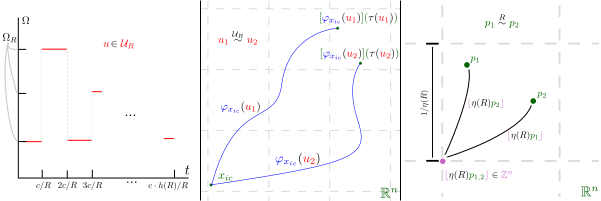
\includegraphics[width=1\textwidth]{Graphics/Theory_Intuition/intuition}
\caption{\label{fig:intuition} Color coded depictions of: (left) a signal from $\mathcal{U}_R$ with signals represented in red, (middle) the mapping into the trajectory space $\mathcal{X}_{x_\mathrm{ic}}$ in blue for two equivalent signals $u_1 \overset{\mathcal{U}_R}{\sim}u_2$, and (right) the mapping from terminal states in $\mathbb{R}^n$ shown in green into $\mathbb{Z}^n$ by the floor map. {\color{red} Nice picture. Would be even better, if the symbols were larger and easier to read.}}
\end{figure}

\subsection{Algorithm Description} 

\mcmargin{Add and introductory sentence explaining what are you going to do in this section, something like: In this section, we are going to propose a specific algorithm called GLC-Search that leverages GLC conditions to achieve guaranteed asymptotic optimality for a very general class of motion planning problems. }{}

Algorithm \ref{Alg} below is a best-first search using the \GLC conditions to discard nonminimal signals and their descendants.
%
\mcmargin{In Algorithm~\ref{Alg} we show the pseudocode of GLC-Search algorithm that performs best-first search while using GLC conditions to discard nonminimal signals and their descendants.}{}
%
A set $Q$ serves as a priority queue of candidate signals. A set $\Sigma$ contains signals representing labels of $\overset{\mathcal{U}_R}{\sim}$ equivalence classes.
 
%
The method $expand(u)$ returns the set of all children of $u$. 
%
The method $pop(Q)$ deletes from Q, and returns an input signal $\hat{u}$ such that 
%
\begin{equation}
\hat{u}\in\underset{u\in Q}{{\rm argmin}}\left\{ J_{x_\mathrm{ic}}(u)\right\}. \label{eq:queue}
\end{equation} 
%
The addition of an admissible heuristic~\cite{hart1968formal} in (\ref{eq:queue}) can be used to guide the search search without affecting the solution accuracy. 
%
\mcmargin{Conveniently, the steering subroutine required by \RRTs is such an admissible heuristic so that Algorithm \ref{Alg} benefits from having this steering function when it is available.}{Its weird that you talk about RRT* in here. I would discuss this in the experimental comparision section.} 

The method $find(u,\Sigma)$ returns $w\in\Sigma$ labeling a region of the partition such that $u\overset{R}{\sim}w$. 
%
If no such $w$ exists then the method returns \NULL. 
%
\mcmargin{Problem-specific}{} Collision and goal checking subroutines are used to evaluate $u\in\mathcal{U}_\mathrm{feas}$ and $u\in\mathcal{U}_\mathrm{goal}$.
%
The method $depth(u)$ returns the number of ancestors of $u$. 
%

 
%
\begin{algorithm} 
\begin{algorithmic}[1]
\State $Q\leftarrow \{Id_\mathcal{U}\},\,\Sigma \gets \emptyset,\,S \gets \emptyset$  
\While {$Q\neq \emptyset$}        
\State $u \gets pop(Q)$   
\State $S \gets expand(u)$   
\For{$w \in S$} 	
\If{$w \in \mathcal{U}_\mathrm{goal} $}         	  
\State \Return $(J(w),w)$ 	
\EndIf       
\State $z = find(w,\Sigma)$ 	  
\If{$(w \notin \mathcal{U}_{feas.} \vee (z \prec_R w) \vee depth(w) \geq h(R))$}  	    
\State $S \gets S\setminus w$  {\color{red} [MC]:$S \gets S\setminus \{w\}$} 	  
\ElsIf{$J_{x_\mathrm{ic}}(w)<J_{x_\mathrm{ic}}(z)$} 	  
\State $\Sigma \gets (\Sigma \setminus {z}) \cup {w}$ {\color{red} [MC]:$\Sigma \gets (\Sigma \setminus \{z\}) \cup \{w\}$} 	
\EndIf 
\EndFor       
\State $Q \gets Q \cup S$ 
\EndWhile  
\State 
\Return $(\infty,NULL)$ {\color{red} [MC]:$(\infty,\texttt{NULL})$} 	
\end{algorithmic} \caption{\label{Alg} Generalized Label Correcting Method} 
\end{algorithm}
%
The algorithm begins by adding the root $Id_\mathcal{U}$ to the queue (line 1), and then enters a loop which terminates if the queue is empty (line 2) \mcmargin{returning NULL}{This sounds like the algorithm will always returns NULL.} (line 14). \mcmargin{Maybe something like: ..., and then enters a loop in which it recursively expands the elements from the top of the queue.}{} At the beginning of an iteration the lowest cost signal in $Q$ is removed (line 3) and its children stored in $S$ (line 4).  Then, each child signal in $S$ (line 5) is checked for membership in $\mathcal{U}_\mathrm{goal}$ in which case the algorithm \mcmargin{found an optimal goal-reaching signal for the given resolution and }{} terminates \mcmargin{ returns the solution, and terminates.}{}. Otherwise, the signal is checked for infeasibility or suboptimality by the \GLC conditions (line 9). If the vertex remains feasible a relabeling condition is checked to see if it should label its repsective equivalence class (line 11). Finally, the children of $u$ which remain are added to the queue (line 13).  

\mcmargin{Otherwise, the child signal is checked for feasibility and GLC conditions are evaluated to verify that the signal is not dominated by the current minimal signal from its equivalence class (line 9). If the child signal has lower cost than the curent label for its equivalence class, then it is used to relabel the equivalence class (line 11). Finally, all feasible and non-dominated children of $u$ are added to the queue (line 13). }{}

\mcmargin{Theorem 1 is the main result of your paper and thus it should stand out. I would put the theorem here, introduced by a very high-level explanation of the idea behind the analysis.}


\mcmargin{Something like: By doing {\em this and that}, as elaborated in detail in Section 4, it is possible to show the following cornerstone property of the GLC-Search algorithm:}


\mcmargin{Theorem 1: ...}


Theorem \ref{thm:main} shows that this algorithm is resolution complete in reference to Problem \ref{Problem}.
This conclusion is independent of the order in which children of the current node are examined in line 5 as well as the relabeling condition in line 11. 
  


\section{\label{sec:Numerical-Examples}Numerical Experiments}

\mcmargin{Again, I would add an introductory sentence trying to explain what are you trying to achieve using the experiments. Something like: In this section we report on the results of our experiments comparing practical performance of the proposed algorithm GLC-Search with the existing state of the art techniques. }{}

\mcmargin{I would very clearly separate results on kinodynamic problems (against SST) and kinematic problems (against RRT*). Where the latter should be presented as a bonus/curiosity. I would put each in its own section. }


Algorithm \ref{Alg} was tested on several problem instances and compared with the \SST and \RRTs \mcmargin{implementations taken from~\cite{rrt_implementation} and~\cite{BBekris2015}}{Did you use their C++ implementation or did you reimplement the algorithm yourself?}. \RRTs is applied only when a closed form expression for the optimal local planner subroutine is available. Observations are discussed at the end of the section.

\paragraph{Implementation Details:}

Algorithm \ref{Alg} was implemented in C++ and run with a 3.70GHz Intel Xeon CPU. 
%
The $pop(Q)$ method was implemented using an STL priority queue for $Q$. 
%
The $find(w,\Sigma)$ method was implemented using an \mcmargin{STL set}{Not very informative in term of complexity. Is it tree or hash set?} for $\Sigma$. 
%
Sets $X_\mathrm{free}$ and $X_\mathrm{goal}$ are \mcmargin{}{} algebraic inequalities, so evaluating $p\in X_\mathrm{free}$ is \mcmargin{trivial}{Vague term. I would leave the comment on the complexity of evaluation out. }.


Evaluation of $u\in\mathcal{U}_\mathrm{feas}$ and $u\in\mathcal{U}_\mathrm{goal}$ is approximated by first numerically approximating $\varphi_{x_\mathrm{ic}}(u)$ with Euler integration. The number of time steps is given by $N=\left\lceil \tau(u)/\Delta\right\rceil $ with duration $\tau(u)/N$. Maximum time steps $\Delta$ are 0.1 for the first two problems and 0.005 in the third. Feasibility is  approximated by uniformly spaced samples along the trajectory,
%
\begin{equation}
u\in\mathcal{U}_\mathrm{feas}\approx\bigwedge_{i=0}^{N}[\varphi_{x_\mathrm{ic}}(u)](i\cdot\tau(u)/N)\in X_\mathrm{free}.\label{eq:collision_checking}
\end{equation}

%
\begin{example}
(Pendulum swing-up) A pendulum is actuated by a torque at the joint. 
%
The problem is to find a torque \mcmargin{history}{control signal} which minimizes the time to reach the inverted position. 
%
The state coordinates consists of the angle and angular rate $(\theta,\omega)$.
%

%
The dynamics are 
%Is it constant time?Is it constanIs it constant time?Is it constant time?t time?
\begin{equation}
\dot{\theta}(t)=\omega(t),\quad\dot{\omega}(t)=-\sin(\theta(t))+u(t),\label{eq:pendulum}
\end{equation}
%
with the torque $u$ limited to $\Omega=[-0.2,0.2]$. 
The initial state $x_{0}$ is $(0,0)$ and the goal region $X_\mathrm{goal}$ is $\{(\theta,\omega):\,\Vert(\theta\pm\pi,\omega)\Vert_{2}<0.1\}$.
%
A minimum-time objective is reflected by the stage cost $g(x,u)=1$ in (\ref{eq:real_cost}).
%
\mcmargin{We run SST algorithm GLC-Search algorithm. The GLC-Search was parametrized as follows: }{}
A uniform discretization of $\Omega$ was used for $\Omega_{R}$,
%
\begin{equation}
\Omega_{R}=\{u\in[-0.2,0.2]:\, u=(0.2i-0.2(R-i))/R,\; i=0,...,R\}.\label{eq:input_disc}
\end{equation}
%
\end{example}
%
%For this system and cost, the relevant Lipschitz constants %are $L_{g}=0$ and $L_{f}=1$. 
%
An ad hoc selection of algorithm parameters satisfying (\ref{eq:h_constraint}) and (\ref{eq:partition_scaling}) was made. These were $c=6$, $\eta(R)=16.0R^{2.5}$, $h(R)=100R\log(R)$. 
%
\mcmargin{The parameters for GLC-Search that satisfy (\ref{eq:h_constraint}) and (\ref{eq:partition_scaling}) were chosen empirically as follows: $c=6$, $\eta(R)=16.0R^{2.5}$, $h(R)=100R\log(R)$.}{}
%
\mcmargin{The parameters used when running SST were: ... are there any parameters in SST?}{}
%
\mcmargin{Numerical results}{Results of the experiment} are summarized in Figure \ref{fig:pendulum}.   

%
\begin{figure}
\centering{}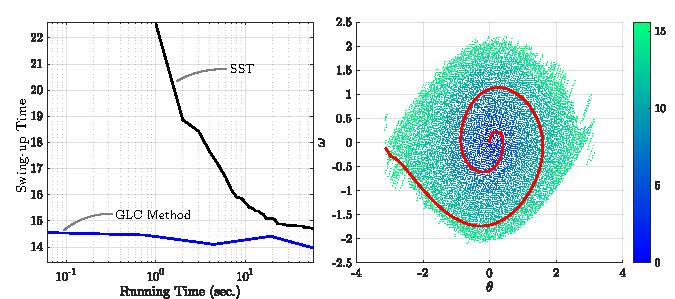
\includegraphics[width=1\textwidth]{Graphics/Pendulum_Example/pendulum}\caption{\label{fig:pendulum} (Left) Cost and running time on a logarithmic time scale of Algorithm \ref{Alg} for resolutions $R\in\{4,5,6,7,8\}$ in blue, and the 10 trial average cost returned by SST in black. There is a notable difference in running times between the \GLC method and \SST. (Right) The colormap indicates cost and associated terminal states of signals in the set of labels $\Sigma$ at the termination of Algorithm \ref{Alg} for $R=6$. {\color{red} Its impossible to tell the two lines when the paper is printed. Can you make one of them dashed? Also, the term GLC Method is not properly defined. I would suggest to give a name to Algorithm 1 (e.g. GLC-Search) and use it to refer to this specific algorithm instead of a little awkward "Algorithm 1".}}
\end{figure}

\begin{example} (Minimum-time acrobot swing-up)
%
The complex dynamics of the acrobot make it a popular benchmark for planning and control techniques.
%
\mcmargin{Acrobot is}{} A two-link pendulum with an actuation torque applied to the second joint \mcmargin{that}{} emulates a gymnast swinging on a bar by applying torque at their hip. 
%
\mcmargin{I would swap the order of the previous two sentences: first explain what is acrobot and than explain why is it popular.}{}
%
The details of the dynamics can be found in the seminal paper by Spong~\cite{spong1995swing}, and are omitted \mcmargin{here}{} for brevity. 
%


%
\mcmargin{The same problem parameters as those used in the problem contained in the SST library are used with the modification that the radius of the goal region is reduced to
0.5 from 2.0 and the integration time-step is set to 0.1.}{It is unclear to me what are you trying to say in that sentence. I would remove it.}
% 

%
Algorithm parameters for this problem were $c=6$, $\eta(R)=16.0R^{2}$, and $h(R)=100R\log(R)$. 
%
Numerical results are summarized in Figure \ref{fig:acro}.
% 
\end{example}
\begin{figure}
\centering{}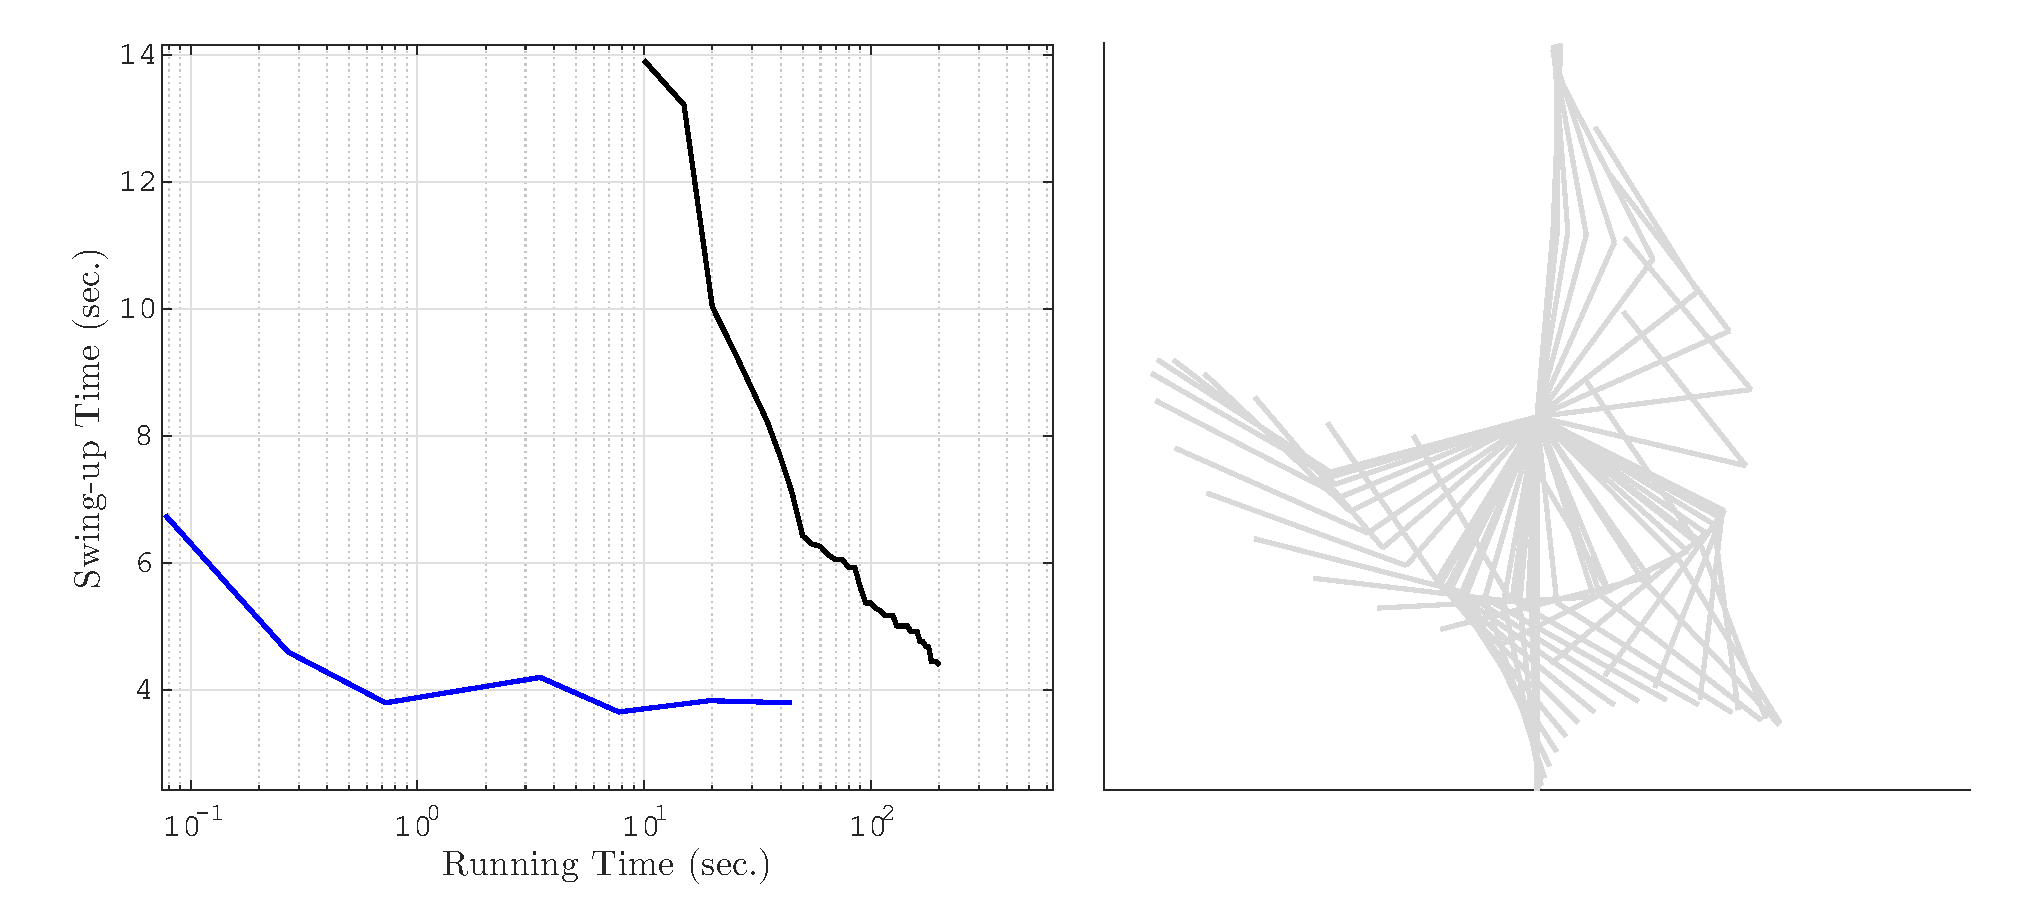
\includegraphics[width=1\textwidth]{Graphics/Acrobot_Example/acro}\caption{\label{fig:acro}(Left) Cost and running time on a logarithmic time scale of Algorithm \ref{Alg} for resolutions $R\in\{4,...,10\}$ in blue, and the 10 trial average cost returned by SST in black. Again, there is a notable difference in running time. (Right) Snapshots of the swing-up motion
returned by Algorithm \ref{Alg} for $R=10$. {\color{red}The same as in Fig 2.}}
\end{figure}

\mcmargin{\subsection{Problems with steering function.}}

\mcmargin{I would clearly argue that this is not your battleground.}

\mcmargin{The proposed algorithm is specifically aimed at kinodynamic motion planning problem, where point-to-point steering function is not available. Many popular existing motion planning algorithms, such as probabilistic roadmaps and RRT*, rely on steering functions that serves as a powerful heuristic allowing more efficient exploration of the state space. In this section we explore the performance of the proposed method on a problem where the steering function is available and compare its the performance against RRT*, a method that leverages the extra information available through the steering function.}


\mcmargin{Explain here what is Guided GLC.}{}


\mcmargin{State parameters for SST, GLC, and RRT*}{}


\begin{example} (Kinematic path planning)
\mcmargin{As an example of a problem, where a steering function is readily available, we consider a shortest path problem.}{}
In order to make a comparison with \RRTs a shortest path problem is considered. The steering subroutine used by \RRTs is simply the line connecting two points. 

%
To fit this problem into our framework we use the model $\dot{x}=u$, with $\Omega=\{u\in\mathbb{R}^{2}:\,\Vert u\Vert_{2}=1\}$.
%
The minimum-time stage cost $g(x,u)=1$ is equivalent to a shortest path objective. 
% 

%
The tuning parameters used for Algorithm \ref{Alg} are $c=10$, $\eta(R)=300R^{2}$, and $h(R)=100R\log(R)$. 
%
Numerical results are illustrated in Figure \ref{fig:kine_example}.
\begin{figure}
\centering{}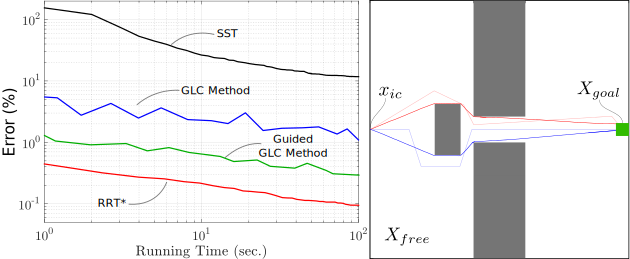
\includegraphics[width=1\textwidth]{Graphics/Kinematic_Example/kine_bench_graphic}\caption{\label{fig:kine_example} (Left) Logarithmic vertical and horizontal axis showing running time and percent error from known optimal cost. Average
running time (10 trials) for the \SST and \RRTs methods are
shown in black and red respectively. Running time of Algorithm \ref{Alg}
is shown in blue for resolutions $R\in\{20,25,...,200\}$. {\color{red} Its not clear if the data points for GLC represent the running time at a particular resolution or sum of running times up to that resolution (which would be fairer).} The guided version of Algorithm \ref{Alg} using the \RRTs steering function is shown in green. (Right) Illustration of the environment. First and last solutions returned by \RRTs are shown red while the first and last solution returned by Algorithm \ref{Alg} are shown in blue.}
\end{figure}
\end{example}

\mcmargin {I would again split discussion for problems without steering function and with steering function.}

\paragraph{Observations and Discussion:}
%
In these problems we observe that the running time of the \GLC method is at least one hundred times faster than the \SST algorithm for a given solution cost. \mcmargin{How can be the difference explained? Even an intuitive attempt to explain the difference in runtime would be nice.}{}

In the third example the \GLC method outperforms \SST but is outperformed by \RRTs. Since the exact solution is known a logarithmic vertical scale is used to observe the convergence rate of each algorithm. Algorithm \ref{Alg} and \RRTs appear to have the same asymptotic convergence rate suggesting that the running time is separated by only a constant factor. 
%
The difference in running time is reduced when using the steering function required by \RRTs as a heuristic to guide the search. 
%
Since the optimal selection of the scaling functions $\eta$ and $h$ has not been investigated it is possible that the gap between the \GLC method and \RRTs can be narrowed further.
%

Note that Algorithm \ref{Alg} terminates in finite time.
%
Each data point in Figures \ref{fig:pendulum}-\ref{fig:kine_example} represents the running time and solution cost of a complete evaluation of the algorithm. 
%
In contrast, \RRTs and \SST are incremental algorithms which run until terminated by the user. 
%	
Each run of Algorithm \ref{Alg} operates on $\mathcal{U}_R$ for a fixed $R$. Since $\mathcal{U}_{R}\not\subset\mathcal{U}_{R+1}$ it is possible that an optimal signal in $\mathcal{U}_R$ may be better than any signal in $\mathcal{U}_{R+1}$ for some $R$ which explains the non-monotonic convergence observed.
%
\section{\label{sec:Justification}Analysis of the GLC Condition}
\mcmargin{I did not go through this section. I believe that reviewers won't be dedicated enough to check the proofs and they will make their mind based the interpretation of the formal results in remaining parts of the paper.}{}

The focus of the remaining discussion is to provide intermediate results to prove that the \GLC method described by Algorithm \ref{Alg} is resolution complete.

We begin with a review of topological properties of the problem data to establish the continuity of the cost functional in \ref{sec:topology}. 
%
This topology is also used to discuss in what sense $\mathcal{U}_R$ approximates $\mathcal{U}$ in Section \ref{sec:discretization}. 
%
The continuity of the cost functional then carries these properties of the approximation of $\mathcal{U}$ into the cost space and ensures that we can approximate an optimal signal. 
%
Finally,  in Lemma \ref{lem:pruning} and Theorem \ref{thm:main}, we derive a bound on the gap between the cost of the solution output by Algorithm \ref{Alg} and the optimal cost for the problem and show that the gap converges to zero as the resolution is increased.


\subsection{Metrics on $\mathcal{X}$ and $\mathcal{U}$, and Continuity of Relevant
Maps \label{sec:topology}}

The metrics introduced by Yershov and Lavalle~\cite{yershov2011sufficient} will be used.  
%
Recall, the signal space $\mathcal{U}$ was defined in (\ref{eq:signal_space}).
A metric on this space is given by 
\begin{equation}
d_{\mathcal{U}}(u_{1},u_{2})\coloneqq\int_{[0,\min(\tau(u_{1}),\tau(u_{2})]}\Vert u_{1}(t)-u_{2}(t)\Vert_{2} \, d\mu(t)+u_{max}|\tau(u_{1})-\tau(u_{2})|.\label{eq:du}
\end{equation}
The family of trajectory spaces are now more precisely defined as 
\begin{equation}
\mathcal{X}_{x_0} \coloneqq \bigcup_{\tau>0}\left\{ x:[0,\tau]\rightarrow \mathbb{R}^n: \: x(0)=x_{0}, \, \left\Vert \frac{x(t_{1})-x(t_{2})}{|t_{1}-t_{2}|}\right\Vert _{2}\leq M\:\, \forall t_{1,2}\in[0,\tau]\right\} ,\label{eq:traj_space}
\end{equation}
where $M$ is that of assumption A-2. This set is equipped with the metric 
\begin{equation}
d_{\mathcal{X}}(x_{1},x_{2})\equiv\max_{t\in\left[0,\min\{\tau(x_{1}),\tau(x_{2})\}\right]}\left\{ \left\Vert x_{1}(t)-x_{2}(t)\right\Vert \right\} +M|\tau(x_{1})-\tau(x_{2})|.\label{eq:traj_metric}
\end{equation}

Several known continuity properties of $\varphi_{x_0}$ are reviewed here. Recall (e.g.~\cite[pg. 95]{khalil1996nonlinear}), that the distance between solutions to (\ref{eq:dynamics}) with initial conditions $x_0$ and $z_0$ is bounded by
\begin{equation}\label{lem:cont_ic}
\left\Vert [\varphi_{x_{0}}(u)](t)-[\varphi_{z_{0}}(u)](t)\right\Vert _{2}\leq\Vert x_{0}-z_{0}\Vert_{2}e^{L_{f}t}.
\end{equation}  

In addition to continuous dependence on the initial condition parameter, the map $\varphi_{x_{0}}$ is also continuous from $\mathcal{U}$ into $\mathcal{X}_{x_{0}}$ (cf.~\cite[Theorem 1]{yershov2011sufficient}). It is a  useful observation then that $\mathcal{X}_\mathrm{feas}$ is open when assumption A-1 is satisfied (cf.~\cite[Theorem 2]{yershov2011sufficient}) since it follows directly from the definition of continuity that $\mathcal{U}_\mathrm{feas}$ and $\mathcal{U}_\mathrm{goal}$ are open subsets of $\mathcal{U}$; recall that they are defined as the preimage of $\mathcal{X}_\mathrm{feas}$ and $\mathcal{X}_\mathrm{goal}$ under $\varphi_{x_\mathrm{ic}}$.

Similar observations for the cost functional are developed below.

\begin{lemma} \label{lem:cost_cont}
%
$J_{x_0}:\mathcal{U}\rightarrow\mathbb{R}$ is continuous for any $x_0\in \mathbb{R}^n$.
%
\end{lemma}
%
\begin{proof}
Let $u_{1},u_{2}\in\mbox{\ensuremath{\mathcal{U}}}$ and without
loss of generality, assume $\tau(u_{1})\leq\tau(u_{2})$. Denote
trajectories $\varphi_{x_{0}}(u_{1})$ and $\varphi_{x_{0}}(u_{2})$ by
$x_{1}$ and $x_{2}$ respectively. The associated difference in cost is 
\begin{equation}
\begin{array}{rl}
\left|J_{x_0}(u_{1})-J_{x_0}(u_{2})\right|= & \left|\int_{\left[0,\tau(u_{1})\right]}g\left(x_{1}(t),u_{1}(t)\right)\right.-g\left(x_{2}(t),u_{2}(t)\right)\, d\mu(t)\\
 & +\left.\int_{\left[\tau(u_{1}),\tau(u_{2})\right]}g\left(x_{2}(t),u_{2}(t)\right)\, d\mu(t)\right|.
\end{array}
\end{equation}
Using the Lipschitz constant of $g$ (cf. A-3), the definition of $d_{\mathcal{U} }$ in (\ref{eq:du}), and the definition of $d_{\mathcal{X} }$ in (\ref{eq:traj_metric}) the difference is bounded as follows: 
\begin{equation}
\begin{array}{rcl}
\left|J_{x_0}(u_{1})-J_{x_0}(u_{2})\right| & \leq & \left|\int_{\left[0,\tau(u_{1})\right]} L_{g}\left\Vert x_{1}(t)-x_{2}(t)\right\Vert _{2}\right.+L_{g}\left\Vert u_{1}(t)-u_{2}(t)\right\Vert _{2}\, d\mu(t) \\
 &  & +\left.\int_{\left[\tau(u_{1}),\tau(u_{2})\right]}g\left(x_{2}(t),u_{2}(t)\right)\, d\mu(t)\right|\\
 & \leq & L_{g}\tau(u_{1})\left\Vert x_{1}-x_{2}\right\Vert _{L_{\infty}\left[0,\tau(u_{1})\right]}+L_{g}\left\Vert u_{1}-u_{2}\right\Vert _{L_{1}\left[0,\tau(u_{1})\right]}\\
 &  & +\int_{\left[\tau(u_{1}),\tau(u_{2})\right]}\left|g\left(x_{2}(t),u_{2}(t)\right)\right|\, d\mu(t)\\
 & \leq & L_{g}\tau(u_{1}) d_{\mathcal{X}}(x_1,x_2)+ L_{g}d_{\mathcal{U}}(u_1,u_2)\\ 
& &  +\int_{\left[\tau(u_{1}),\tau(u_{2})\right]}\left|g\left(x_{2}(t),u_{2}(t)\right)\right|\, d\mu(t). 
\end{array}\label{eq:cost_diff}
\end{equation}
Since $x_2$ is continuous, $u_2$ is bounded, and $g$ is continuous, there exists a bound $G$ on $g(x_2(t),u_2(t))$ for $t\in [\tau(u_1),\tau(u_2)]$. Thus, the difference in cost is further bounded by  

\begin{equation}
\begin{array}{rcl}
\left|J_{x_0}(u_{1})-J_{x_0}(u_{2})\right| & \leq & L_{g}\tau(u_{1}) d_{\mathcal{X}}(x_1,x_2) + L_{g}d_{\mathcal{U}}(u_1,u_2) +G(\tau(u_2)-\tau(u_1)). 
\end{array}
\label{eq:cost_diff2}
\end{equation}
From the continuity of $\varphi_{x_0}$, for $d_{\mathcal{U}}(u_1,u_2)$ sufficiently small the resulting trajectories will satisfy $L_{g}\tau(u_{1}) d_{\mathcal{X}}(x_1,x_2)<\varepsilon/3$. For $u_1,u_2$ additionally satisfying $d_{\mathcal{U}}(u_1,u_2)<\frac{\varepsilon u_{max}}{3G}$ and $d_{\mathcal{U}}(u_1,u_2)<\frac{\varepsilon}{3L_g}$ we have $G(\tau(u_2)-\tau(u_1))<\varepsilon/3$  and $L_{g}d_{\mathcal{U}}(u_1,u_2)<\varepsilon/3$. For such a selection of $u_1,u_2$, we have $|J_{x_0}(u_1)-J_{x_0}(u_2)|<\varepsilon$. Thus, $J_{x_0}$ is continuous.
\qed
\end{proof} 
\begin{lemma}
\label{lem:cost_sensitivity}For any $u\in\mathcal{U}_\mathrm{feas}$ and
$x_{0},z_{0}\in\mathbb{R}^{n}$, 
\begin{equation}
|J_{x_{0}}(u)-J_{z_{0}}(u)|\leq\Vert x_{0}-z_{0}\Vert_{2}\cdot\frac{L_{g}}{L_{f}}\left(e^{L_{f}\tau(u)}-1\right)\label{eq:cost_sensitivity}
\end{equation}
\end{lemma}
\begin{proof}
The difference is bounded using the Lipschitz continuity of $g$. This is further bounded using (\ref{lem:cont_ic}). Denoting $x(t)=\varphi_{x_{0}}(u)$ and $z(t)=\varphi_{z_{0}}(u)$,
\begin{equation}
\begin{array}{rcl}
|J_{x_{0}}(u)-J_{z_{0}}(u)| & = & \left|\int_{[0,\tau(u)]}g(x(t),u(t))\right. \left.-g(z(t),u(t))\, d\mu(t) \right|\\
 & \leq & \int_{[0,\tau(u)]}\left|g(x(t),u(t))\right. \left.-g(z(t),u(t))\right|\, d\mu(t)\\
 & \leq & \int_{[0,\tau(u)]}L_{g}\left\Vert x(t)-z(t)\right\Vert _{2}\, d\mu(t)\\
 & \leq & \int_{[0,\tau(u)]}\Vert x_{0}-z_{0}\Vert_{2} L_{g}e^{L_{f}t}\, d\mu(t)\\
 & = & \Vert x_{0}-z_{0}\Vert_{2}\frac{L_{g}}{Lf}\left(e^{L_{f}\tau(u)}-1\right).
\end{array}
\end{equation}
 \qed
\end{proof}

\subsection{Properties of the Approximation of $\mathcal{U}$ by $\mathcal{U}_{R}$ \label{sec:discretization}}

%The next two results examine in what sense elements of %$\mathcal{U}$ are approximated by elements of %$\mathcal{U}_R$, and together with the continuity of the cost function, how these signals can approximate the optimal cost. 

Note that Lemma \ref{lem:density} is not a statement about the dispersion of $\mathcal{U}_R$ in $\mathcal{U}$ which does not actually converge. For numerical approximations of function spaces the weaker statement that $\limsup_{R\rightarrow \infty}\mathcal{U}_R$ is dense in $\mathcal{U}$ will be sufficient. Equivalently,
%
\begin{lemma}
\label{lem:density}For each $u\in\mathcal{U}$ and $\varepsilon>0$,
there exists $R^{*}>0$ such that for any $R>R^{*}$ there exists
$w\in\mathcal{U}_{R}$ such that $d_{\mathcal{U}}(u,w)<\varepsilon$.\end{lemma}
\begin{proof}
%The signal $u$ will first be approximated by a uniformly continuous
%function $\omega$, and then $w\in\mathcal{U}_{R}$ will be constructed
%to approximate $\omega.$ 

By Lusin's Theorem~\cite[pg. 41]{kolmogorov1961elements}, there exists
a continuous $\upsilon:[0,\tau(u)]\rightarrow\Omega$ such that 
\begin{equation}
\mu(\{t\in[0,\tau(u)]:\:\upsilon(t)\neq u(t)\})<\frac{\varepsilon}{3u_{max}}.
\end{equation}
The domain of $\upsilon$ is compact so $\upsilon$ is also uniformly continuous. Denote its modulus of continuity by $\delta(\epsilon)$,
\begin{equation}
|\sigma-\gamma|<\delta(\epsilon)\Rightarrow\Vert\upsilon(\sigma)-\upsilon(\gamma)\Vert_{2}<\epsilon.
\end{equation}


To construct an approximation of $\upsilon$ by $w\in\mathcal{U}_{R}$
choose $R$ sufficiently large so that (i) $h(R)/R>\tau(u)$,
(ii) there exists an integer $r$ such that $0<\tau(u)-r/R<1/R<\delta\left(\frac{\varepsilon}{6\tau(u)}\right)$,
and (iii) the dispersion of $\Omega_{R}$ in $\Omega$ is less than $\frac{\varepsilon}{6\tau(u)}$. 

Then for $t\in[(i-1)/R,i/R)$ $i=1,...,r$ there exists ${\rm v}_{i}\in\Omega_{R}$
such that $\Vert {\rm v}_{i}-\upsilon(t)\Vert_{2}<\frac{\varepsilon}{3\tau(u)}.$
Select $w\in\mathcal{U}_{R}$ which is equal to ${\rm v}_{i}$ on
each interval. Combining (i)-(iii), 
\begin{equation}
\begin{array}{rcl}
d_{\mathcal{U}}(\upsilon,w) & = & \int_{[0,r/R]}\Vert w(t)-\omega(t)\Vert_{2},\, d\mu(t)+u_{max}|r/R-\tau(\omega)|\\
 & < & \int_{[0,r/R]}\Vert w(t)-\omega(t)\Vert_{2},\, d\mu(t)+\frac{\varepsilon}{6}\\
 & < & \int_{[0,r/R]}\frac{\varepsilon}{3\tau(u)},\, d\mu(t)+\frac{\varepsilon}{6}\\
 & < & \frac{\varepsilon}{2}.
\end{array}
\end{equation}
Thus, by the triangle, inequality
\begin{equation}
d_{\mathcal{U}}(u,w)\leq d_{\mathcal{U}}(u,\upsilon)+d(\upsilon,w)<\varepsilon.
\end{equation}
\qed
\end{proof}

We use $cl(\cdot)$ and $int(\cdot)$ to denote the closure and interior of subsets of $\mathcal{U}$.
\begin{lemma}
\label{lem:no_limit_points}For any $w\in cl\left(int\left(\mathcal{U}_\mathrm{goal}\right)\right)$
and $\varepsilon>0$ there exists $R^{*}>0$ such that for any $R>R^{*}$
\begin{equation}
\min_{u\in\mathcal{U}_{R}\cap\mathcal{U}_\mathrm{goal}}\left\{ \left|J_{x_\mathrm{ic}}(u)-J_{x_\mathrm{ic}}(w)\right|\right\} <\varepsilon.
\end{equation}
\end{lemma}
\begin{proof}
$\omega\in cl\left(int\left(\mathcal{U}_\mathrm{goal}\right)\right)$ implies
that for all $\delta>0$, $B_{\delta/2}(\omega)\cap int(\mathcal{U}_\mathrm{goal})\neq\emptyset$.
Then each $\upsilon\in int(\mathcal{U}_\mathrm{goal})$ has a neighbourhood
$B_{\rho}(\upsilon)\subset int(\mathcal{U}_\mathrm{goal})$ with $\rho<\frac{\delta}{2}$.
Take $\upsilon\in B_{\delta/2}(\omega)\cap int(\mathcal{U}_{goal.})$.
By Lemma \ref{lem:density}, for sufficiently large $R$, there exists $u\in\mathcal{U}_{R}$ such
that $d_{\mathcal{U}}(\upsilon,u)<\delta/2$ which implies $u\in B_{\rho}(\upsilon)\subset int(\mathcal{U}_\mathrm{goal})$.
Then $u\in\mathcal{U}_\mathrm{goal}$ and $d_{\mathcal{U}}(\omega,u)<d_{\mathcal{U}}(\omega,\upsilon)+d_{\mathcal{U}}(\upsilon,u)<\delta$. Now by the continuity of $J_{x_\mathrm{ic}}$ for $\delta$ sufficiently small, $d_{\mathcal{U}}(\omega,\upsilon)<\delta$ implies $|J_{x_\mathrm{ic}}(u)-J_{x_\mathrm{ic}}(w)| <\varepsilon$ from which the result follows.
\qed
\end{proof}
A sufficient condition for every $\omega\in\mathcal{U}_\mathrm{goal}$ to
be contained in the closure of the interior of $\mathcal{U}_\mathrm{goal}$ is that $\mathcal{U}_\mathrm{goal}$ be open which is the case when Assumption A-1 is satisfied. 
%
%In connection to the framework of %~\cite{karaman2011sampling,Li2016Asymptotically-}, a problem is %$\delta$-robustly feasible iff $cl(int(\mathcal{U}_\mathrm{goal}))\neq %emptyset$.    


\subsection{Pruning $\mathcal{U}_{R}$ with the GLC Condition \label{sec:pruning}}

To describe trajectories remaining on an the $\varepsilon$-interior of $X_\mathrm{free}$ at each instant and which terminate on the $\varepsilon$-interior of $X_\mathrm{goal}$ the following sets are defined,
\begin{equation}
\begin{array}{l}
\mathcal{X}_\mathrm{goal}^{\varepsilon}\coloneqq\left\{ x\in\mathcal{X}_\mathrm{goal}:\,\; B_{\varepsilon}(x(t))\subset X_\mathrm{free}\, \forall t\in[0,\tau(x)], \, B_{\varepsilon}(x(\tau(x))\subset X_\mathrm{goal}\right\} ,\\
\mathcal{U}_\mathrm{goal}^{\varepsilon}\coloneqq\left\{ u\in\mathcal{U}_\mathrm{goal}:\,\varphi_{x_\mathrm{ic}}(u)\in\mathcal{X}_\mathrm{goal}^{\varepsilon}\right\} ,
\end{array}\label{eq:interiors}
\end{equation}
and similarly for $c_{R}$,
\begin{equation}
c_{R}^{\varepsilon}\coloneqq\min_{u\in\mathcal{U}_{R}\cap\mathcal{U}_\mathrm{goal}^{\varepsilon}}\left\{ J_{x_\mathrm{ic}}(u)\right\} .\label{eq:cr_ep}
\end{equation}
 Since $\ensuremath{\mathcal{U}_\mathrm{goal}^{\varepsilon}\subset\mathcal{U}_\mathrm{goal}}$
we have that $0\leq c_{R}\leq c_{R}^{\varepsilon}$. 
\begin{lemma}
\label{lem:approx_equal_optimal}If $\lim_{R\rightarrow\infty}\epsilon(R)=0$
then $\lim_{R\rightarrow\infty}c_{R}^{\epsilon(R)}=c^{*}$.\end{lemma}
\begin{proof}
By the definition of $c^{*}$ in (\ref{eq:meaningful_problem}), for any
$\varepsilon>0$ there exists $\omega\in\mathcal{U}_\mathrm{goal}$ such
that $J_{x_\mathrm{ic}}(\omega)-\varepsilon/2<c^{*}$. Since
$\mathcal{U}_\mathrm{goal}$ is open and $\varphi_{x_\mathrm{ic}}$ is continuous there exists $\tilde{r}>0$ and $\rho>0$
such that $B_{\tilde{r}}(\omega)\subset\mathcal{U}_\mathrm{goal}$ and $\varphi_{x_\mathrm{ic}}(B_{\tilde{r}}(\omega))\subset B_{\rho}(\varphi_{x_\mathrm{ic}}(\omega))$.
Thus, $\omega\in\mathcal{U}_\mathrm{goal}^{\tilde{r}}$. Similarly, there exists a positive $r<\tilde{r}$ such that $\varphi_{x_\mathrm{ic}}(B_{r}(\omega))\subset B_{\rho/2}(\varphi_{x_\mathrm{ic}}(\omega))$
and $B_{r}(\omega)\subset\mathcal{U}_\mathrm{goal}^{\rho/2}$. From the continuity
of $J$ in Lemma \ref{lem:cost_cont} there also exists a positive
$\delta<r$ such that for any signal $\upsilon$ with $d_{\mathcal{U}}(\upsilon,\omega)<\delta$
we have $|J_{x_\mathrm{ic}}(\omega)-J_{x_\mathrm{ic}}(\upsilon)|<\varepsilon/2$.

Next, choose $R^{*}$ to be sufficiently large such that $R>R^*$ implies $\mbox{\ensuremath{\epsilon}}(R)<\rho/2$
and $B_{\delta}(\omega)\cap\mathcal{U}_{R}\neq\emptyset$. Such a resolution $R^{*}$ exists by
Lemma \ref{lem:no_limit_points} and the assumption $\lim_{R\rightarrow\infty}\epsilon(R)=0$.
Now choose $u\in B_{\delta}(\omega)\cap\mathcal{U}_{R}$.
Then $|J_{x_\mathrm{ic}}(u)-J_{x_\mathrm{ic}}(\omega)|<\varepsilon/2$ and $u\in\mathcal{U}_\mathrm{goal}^{\rho/2}\subset\mathcal{U}_\mathrm{goal}^{\epsilon(R)}$.
Then by definition of $c_{R}^{\epsilon(R)}$, $u\in\mathcal{U}_\mathrm{goal}^{\epsilon(R)}$
implies $c_{R}^{\epsilon(R)}\leq J_{x_\mathrm{ic}}(u)$. Finally, by triangle
inequality, 
\begin{equation}
|J_{x_\mathrm{ic}}(u)-c^{*}|<|J_{x_\mathrm{ic}}(u)-J_{x_\mathrm{ic}}(\omega)|+|J_{x_\mathrm{ic}}(\omega)-c^{*}|<\varepsilon.
\end{equation}
Rearranging the expression yields $J_{x_\mathrm{ic}}(u)<c^{*}+\varepsilon$
and thus, $c_{R}^{\epsilon(R)}<c^{*}+\varepsilon$. The result follows
since the choice of $\varepsilon$ is arbitrary.
\qed
\end{proof}

To simplify the notation in what follows, a concatenation operation on elements of $\mathcal{U}$ is defined.
For $u_{1},u_{2}\in\mathcal{U}$, their concatenation $u_{1}u_{2}$
is defined by 
\begin{equation}
[u_{1}u_{2}](t)\coloneqq\left\{ \begin{array}{c}
u_{1}(t),\, t\in[0,\tau(u_{1}))\\
u_{2}(t-\tau(u_{1})),\, t\in[\tau(u_{1}),\tau(u_{1})+\tau(u_{2})]
\end{array}\right..\label{eq:concatenation}
\end{equation}
%
The concatenation operation will be useful together
with the following equalities which are readily verified, 
\begin{equation}\label{eq:cost_homo}
J_{x_{0}}(u_{1}u_{2})=J_{x_{0}}(u_{1})+J_{[\varphi_{x_0}(u_1)](\tau(u_1))}(u_{2})
\end{equation}
\begin{equation}
\ensuremath{\varphi_{x_{0}}(u_{1}u_{2})=\varphi_{x_{0}}(u_{1})\varphi_{[\varphi_{x_{0}}(u_1)](\tau(u))}(u_{2})}.\label{eq:x_concat}
\end{equation}
The concatenation operation on $\mathcal{X}_{x_{0}}$ in (\ref{eq:x_concat})
is defined in the same way as in (\ref{eq:concatenation}). 
\begin{lemma}
\label{lem:pruning}Let $\delta_0=\frac{\sqrt{n}}{\eta(R)}e^{\frac{L_{f}h(R)}{R}}$.
For $\varepsilon\geq \delta_0$ and $u_{i},u_{j}\in\mathcal{U}_{R}\cap\mathcal{U}_\mathrm{feas}$, if
$u_{i}\prec_{R}u_{j}$, then for each descendant of $u_{j}$ in $\mathcal{U}_\mathrm{goal}^{\varepsilon-\delta_0}$
with cost $c_{j}$, there exists a descendant of $u_{i}$ in $\mathcal{U}_\mathrm{goal}$
with cost $c_{i}\leq c_{j}$.\end{lemma}
\begin{proof}
Suppose there is a $w\in\mathcal{U}_{R}$ such that $u_{j}w\in\mathcal{U}_{R}$
is a descendant of $u_{j}$ and $u_{j}w\in\mathcal{U}_\mathrm{goal}^{\varepsilon}.$
 Since $u_{i}\overset{R}{\sim}u_{j}$,
\begin{equation}
\left\Vert[\varphi_{x_\mathrm{ic}}(u_{i}w)](\tau(u_{i}))-[\varphi_{x_\mathrm{ic}}(u_{j}w)](\tau(u_{j}))\right\Vert_2\leq \frac{\sqrt{n}}{\eta(R)}.
\end{equation}
Then, by equation (\ref{lem:cont_ic}), for all $t\in[0,\tau(w)]\subset[0,h(R)/R]$, 
\begin{equation}
\Vert[\varphi_{x_\mathrm{ic}}(u_{i}w)](t+\tau(u_{i}))-[\varphi_{x_\mathrm{ic}}(u_{j}w)](t+\tau(u_{j}))\Vert\leq\frac{\sqrt{n}}{\eta(R)}e^{\frac{L_{f}h(R)}{R}}.\label{eq:-8}
\end{equation}
Then for $\delta_0=\frac{\sqrt{n}}{\eta(R)}e^{\frac{L_{f}h(R)}{R}}$
we have $u_{i} w \in \mathcal{U}_\mathrm{goal}^{\varepsilon-\delta_0}.$ 
As for the cost, from equation (\ref{eq:cost_homo}) 
\begin{equation}
\begin{array}{rcl}
J_{x_\mathrm{ic}}(u_{i} w) & = & J_{x_\mathrm{ic}}(u_{i})+J_{[\varphi_{x_\mathrm{ic}}(u_{i})](\tau(u_{i}))}(w)\\
 & \leq & J_{x_\mathrm{ic}}(u_{j})+\frac{\sqrt{n}}{\eta(R)}\frac{L_{g}}{L_{f}}\left(e^{\frac{L_{f}h(R)}{R}}-1\right) +J_{[\varphi_{x_\mathrm{ic}}(u_{j})](\tau(u_{j}))}(w)\\
 & \leq & J_{x_\mathrm{ic}}(u_{j})+J_{[\varphi_{x_\mathrm{ic}}(u_{j})](\tau(u_{j}))}(w)\\
 & \leq  & J_{x_\mathrm{ic}}(u_{j}w)\\
\end{array}
\end{equation}
 The first step applies the conditions for $u_{i}\prec_{R}u_{j}$.
The second step combines Lemma \ref{lem:cost_sensitivity} and $u_{i}\overset{N}{\sim}u_{j}$. 
\qed
\end{proof}
In the above Lemma, the quantity $\delta_0$ was constructed based on the radius of the partition of $X_\mathrm{free}$ and the sensitivity of solutions to initial conditions. 
%
%
Let $\delta_k$ be defined as a finite sum of related quantities, $\delta_k\coloneqq\sum_{i=1}^{k}\frac{\sqrt{n}}{\eta(R)}e^{\frac{L_{f}(h(R)-i)}{R}}$. The following bound will be useful to state our main result in the next Theorem,
\begin{equation}
\delta_{h(R)}=\sum_{i=1}^{h(R)}\frac{\sqrt{n}}{\eta(R)}e^{\frac{L_{f}(h(R)-i)}{R}} \leq\frac{R\sqrt{n}}{L_{f}\eta(R)}\left(e^{L_{f}h(R)/R}-1\right).\label{eq:inequality}
\end{equation}
This is derived as follows 
\begin{equation}
\begin{array}{rcl}
\sum_{i=1}^{h(R)}\frac{\sqrt{n}}{\eta(R)}e^{\frac{L_{f}(h(R)-i)}{R}} & = & \frac{\sqrt{n}}{\eta(R)}\sum_{i=0}^{h(R)-1}e^{\frac{L_{f}i}{R}}\\
 & \leq & \frac{\sqrt{n}}{\eta(R)}\int_{0}^{h(R)}e^{\frac{L_{f}}{R}\rho}d\rho\\
 & = & \frac{R\sqrt{n}}{L_{f}\eta(R)}\left(e^{\frac{L_{f}h(R)}{R}}-1\right).
\end{array}
\end{equation}
\begin{theorem}\label{thm:main}
Let $\epsilon(R)=\frac{R\sqrt{n}}{L_{f}\eta(R)}\left(e^{\frac{L_{f}h(R)}{R}}-1\right)$. Algorithm \ref{Alg} terminates in finite time and returns a solution with cost less than or equal to $c^{\epsilon(R)}_R$.
\end{theorem}
%
\begin{proof}
The queue is a subset of $\mathcal{U}_R\cup \{Id_\mathcal{U} \}$ and at line 3 in each iteration a lowest cost signal $u$ is removed from the queue. 
%
Observe that any $w$ from the finite set $\mathcal{U}_R$ enters the queue at most once since $w$ is not a child of itself and only children of $w$ enter the queue in line 13. 
%
Therefore the queue must be empty after a finite number of iterations so the algorithm terminates.

Next, as a point of contradiction consider the hypothesis that the output has cost greater than $c_R^{\epsilon(R)}$. 
%
Then $c_R^{\epsilon(R)}<\infty$ and by the definition of  $c_R^{\epsilon(R)}$  in (\ref{eq:cr_ep}), it is necessary that $\mathcal{U}_{R}\cap \mathcal{U}_\mathrm{goal}^{\epsilon(R)}$ is non-empty. 

Signals $u_0\in \mathcal{U}_{R}\cap\mathcal{U}_\mathrm{goal}^{\epsilon(R)}$ with cost $J_{x_\mathrm{ic}}(u_0)=c_R^{\epsilon(R)}$ are descendants of $Id_\mathcal{U}$ which is initially present in the queue. 
%
The hypothesis prohibits these signals from entering the queue. Otherwise, by (\ref{eq:queue}) they would be evaluated before any signal of cost greater than $c_R^{\epsilon(R)}$.To prevent these signals from entering the queue a signal $u_1$  with $depth(u_1)\geq 1$ must at some iteration be present in $\Sigma$ with $u_1 \prec_R a_0$ for an ancestor $a_0$ of each $u_0$. 
%
By line 10, having $u_1$ present in $\Sigma$ allows signals in the sub-tree rooted at $a_0$ containing each $u_0$ to be prevented from entering the queue. 
%
From Lemma \ref{lem:pruning}, each $u_1$ has a descendant in $\mathcal{U}_R$ of the form $u_1d_1$ such that $u_1d_1\in \mathcal{U}_\mathrm{goal}^{\epsilon(R)-\delta_1}$ and $J_{x_\mathrm{ic}}(u_1d_1)\leq c_R^{\epsilon(R)-\delta_1}$. 
%
To be present in $\Sigma$, a signal $u_1$ must at some point be present in the queue as well by line 10. 
%
The hypothesis implies that $u_1d_1$ does not enter the queue which is only possible by the same mechanism as for $u_0$.
%
%The signal $u_1$ must at some point enter the queue since $u_1\in\Sigma$ (line 13). but the hypothesis implies that some ancestor $a_2$ of $u_1d_1$ with $depth(a_1)\geq 2$ must be discarded in the same way as $u_0$

%Since $u_1\in\Sigma$, it must at some point enter the queue (line 13). 
%
%With a descendant violating the hypothesis, there at some point must exist $u_2\in \Sigma $ with $depth(u_2)\geq 2$ such that $u_2\prec_R a_2$ for some ancestor $a_2$ of $u_1d_1$ so that the sub-tree rooted at $u_1d_1$ does not enter the queue. 
%
%Again by Lemma \ref{lem:pruning} each such $u_2$ has a descendant $u_2d_2\in\mathcal{U}_\mathrm{goal}^{\epsilon(R)-\delta_2}$ with $J(u_2d_2,x_\mathrm{ic})\leq c_R^{\epsilon(R)}$. 

Suppose that repeating the process $k<h(R)$ times reveals that a signal $u_k$ with $depth(u_k)\geq k$ must at some iteration be present in the queue and that there is a descendant  $u_kd_k\in\mathcal{U}_R\cap\mathcal{U}_\mathrm{goal}^{\epsilon(R)-\delta_k}$  with cost $J_{x_\mathrm{ic}}(u_kd_k)\leq c_R^{\epsilon(R)}$.
%
Note, $\delta_k \leq \epsilon(R) $ for any $k \leq h(R)$ by (\ref{eq:inequality}).
%
The hypothesis implies that an ancestor $a_{k}$ of $u_kd_k$ must be prevented from entering the queue in lines 9-10 by evaluating $u_{k+1}\prec_R a_{k}$ for some $u_{k+1}\in \Sigma$ with $depth(u_{k+1})\leq k+1$. 
%
Again, by Lemma \ref{lem:pruning}, a descendant of $u_{k+1}$ of the form $u_{k+1}d_{k+1}$ will be in $\mathcal{U}^{\epsilon(R)-\delta_{k+1}}_\mathrm{goal}$ with cost $J_{x_\mathrm{ic}}(u_{k+1}d_{k+1})\leq c_R^{\epsilon(R)-\delta_{k+1}}$ so that some anscestor of $u_{k+1}d_{k+1}$ must be prevented from entering the queue. 

By induction on $k$ we conclude that this procedure can continue up to $k=h(R)$ at which point we find it necessary that there exist signals $u_{h(R)}$ with $depth(u_{h(R)})= h(R)$ such that $u_{h(R)}\prec_R u_{h(R)-1}d_{h(R)-1}$ for the descendant of $u_{h(R)-1}$ in $\mathcal{U}^{\epsilon(R)-\delta_{h(R)-1}}_\mathrm{goal}$. By Lemma \ref{lem:pruning} $u_{h(R)}\prec_R u_{h(R)-1}d_{h(R)-1}$ implies $u_{h(R)}$ has a descendant in $\mathcal{U}_\mathrm{goal}$. However, $u_{h(R)}$ has no descendants-a contradiction.   


\qed
\end{proof}
%

The choice of $\epsilon(R)$ in Theorem \ref{thm:main} converges to zero by  (\ref{eq:partition_scaling}).
%
Then by Lemma \ref{lem:approx_equal_optimal} we have $c_{R}^{\epsilon(R)}\rightarrow c^{*}$. 
%
 An immediate corollary is Algorithm \ref{Alg} is resolution complete.

\section{Conclusion\label{sec:Conclusions}}
%

\mcmargin{In this paper we focused on the problem of designing an efficient, asymptotically optimal algorithm for kinodynamic motion planning that does not require point-to-point steering function.}{}
Our purpose has been to develop an optimal kinodynamic motion planning algorithm that is computationally efficient, provably resolution complete, and does not require a \mcmargin{local planning subroutine}{point-to-point steering function}. 

Inspired by the effectiveness of label correcting methods, efficiency was achieved by generalizing the labeling technique with the \GLC conditions. 
%
A novel approach to the theoretical investigation led us to the conclusion that this algorithm is in fact resolution complete. 
\mcmargin{We provided rigorous theoretical analysis of the new algorithm showing that the algorithm is asymptotically optimal, i.e. .... .}


\mcmargin{Explicitly list the improvements over the existing state of the art:}{}

\mcmargin{Compared to SST, the state-of-the-art method for kinodynamic motion planning without steering function, the proposed algorithm relaxes assumptions on .... which is useful e.g. in problem that ... .}{}

\mcmargin {Moreover, in experimental analysis, we have demonstrated that the proposed algorithm is by multiple orders of magnitude faster than SST.}

%
The distinct approach even allowed us to omit the weakened controllability assumption required by \RRTs and \SST.    
%
  
%The \GLC method described by Algorithm \ref{Alg} was implemented and compared in several examples to the \SST algorithm, and the \RRTs algorithm for a kinematic example.
%
%In the kinematic example for which \RRTs is specialized, we observed that the convergence rate appeared to be the same suggesting a difference in running time by only a constant factor.
%
%In comparison to \SST in both kinematic and kinodynamic examples, the \GLC method obtained solutions of a given cost no less than 100 times faster than \SST in each experiment. 


From a practical point of view, the proposed algorithm may be used directly, but several \mcmargin{interesting questions remain}{This sounds negative. I would remove. Instead I would say something like: In future, we plan to focus on principled selection and optimization of the parameters of the algorithm that may enable further performance improvements.}. 
%
In particular, the selection of the scaling parameters $c$, $\eta$, $h$, and the geometry of the partition of $X_\mathrm{free}$ has been somewhat arbitrary and a careful study may reveal optimal values to achieve the best performance for the algorithm.
\section*{Acknowledgements}
This research was funded in part by the Israeli Ministry of Defense. 
\bibliographystyle{splncs}
\bibliography{references}

\end{document}